\section{Errores}

Este es un ejercicio que en el González no está debidamente explicado.

Calcular con tres decimales correctos o significativos la siguiente expresión: $$x=a\, \pi$$ siendo $\bar{a} = 1.3134$.

De acuerdo con lo convenido, asumimos que 1.3134 está correctamente redondeado, por lo tanto su error absoluto inherente es menor o igual que $0.5\e{-4}$.
Por otro lado el problema numérico planteado propagará los errores inherentes de acuerdo a la siguiente expresión:
\[e_x = \pi \, e_{a} + a\, e_{\pi}\]

Tres decimales correctos o significativos significa de acuerdo a la Convención 4.2 que el error absoluto del resultado obtenido debe ser menor o igual, en módulo, a $0.5\e{-3}$; por lo tanto nuestro objetivo es que:

\[ \left| e_x \right| \le 0.5\e{-3} \]

Por la desigualdad triangular:

\[ \left| e_x \right| \le \left| \pi \, e_{a} \right| + \left| a \, e_{\pi}    \right|  \le 0.5\e{-3}  \]

Acoto $\pi \le 3.15$, y $a\le 1.3135$, pues asumo que está bien redondeado (el valor real  $a \in [1.31335; 1.313450)$). Podría también haber usado algo un poco más fino, como $\pi \le 3.1316$ y $a\le 1.313450$, pero dado que estoy estimando una cota no necesito demasiada precisión --más adelante quedará más claro--. En fin:

\[ \left| e_x \right| \le  3.15 \cdot 0.5\e{-4}  +  1.3135\, |e_{\pi}|      \le 0.5\e{-3}  \]

Y despejando: 

\[ \left| e_{\pi} \right| \le  \frac{0.5\e{-3} - 0.5 \e{-4} \cdot 3.15 }{1.3135} \simeq 2.61 \e{-4} \]

Ahora que tenemos esta cota ¿cuántos decimales se necesitan? Necesito la \emph{mínima} cantidad de decimales que me aseguren un error menor o igual a ese. Como uso redondeo, el error es de la forma $e = 0.5\e{-n}$, con $n$ la cantidad de decimales. Dado que $|e_{\pi}| \le 0.261\e{-3}$, podemos acotar:

$$|e_{\pi}| \le 0.5\e{-n} \le 0.261\e{-3}$$

Y despejar entonces: $n\ge4$. Esto mismo se observa en la Figura \ref{fig:g1:errores_cantidad_decimales}.

\begin{figure}
	\centering
	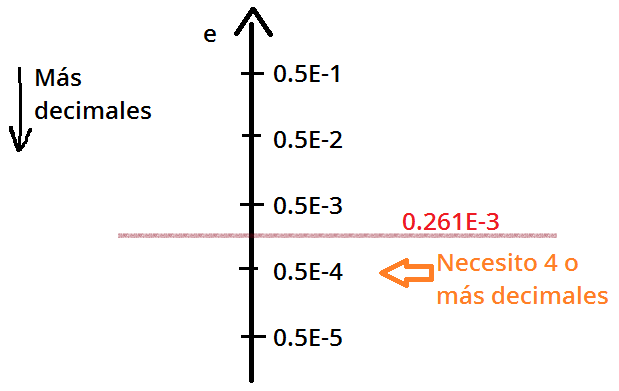
\includegraphics[width=0.4\linewidth]{guia1/errores_cantidad_decimales}
	\caption{Cantidad de decimales y errores inherentes en punto fijo con redondeo.}
	\label{fig:g1:errores_cantidad_decimales}
\end{figure}


De donde deducimos que usando $\pi$ con cuatro decimales significativos y no cometiendo errores apreciables de redondeo en el producto, $\bar{x}$ tendrá tres decimales correctos o significativos, o sea, como:

\[1.3134\cdot 3.1416 = 4.1261774\text{, resulta }x=4.1261774 \pm 0.0005\]

o mejor aún:

\[\bar{x} = 4.126\]

